\subsection{Overall Accuracy or true positive}\label{4.1.1}
In this section we tested the algorithms using the transformed test dataset. The test datatsets were applied with increasing value of transformations identified in \ref{identifyingMR}. A copy of these new datasets generated from the original dataset by applying the transformations were saved to serve as follow-up test cases. For example, the MNIST dataset was transformed by applying the shading metamorphic relation for every pixel between [-28,28]. The models were then tested with transformed test data and their accuracy were calculated for every follow-up test data. The following graphs shows the change in accuracy of the whole dataset as the degree of transformation is changed. The X-axis shows the value of metamorphic transformation applied to the original test data and the Y-axis shows the accuracy corresponding to that value of transformation.
    \begin{figure}[htb!]
    \centering
    \begin{subfigure}[b]{0.3\textwidth}
        \centering
        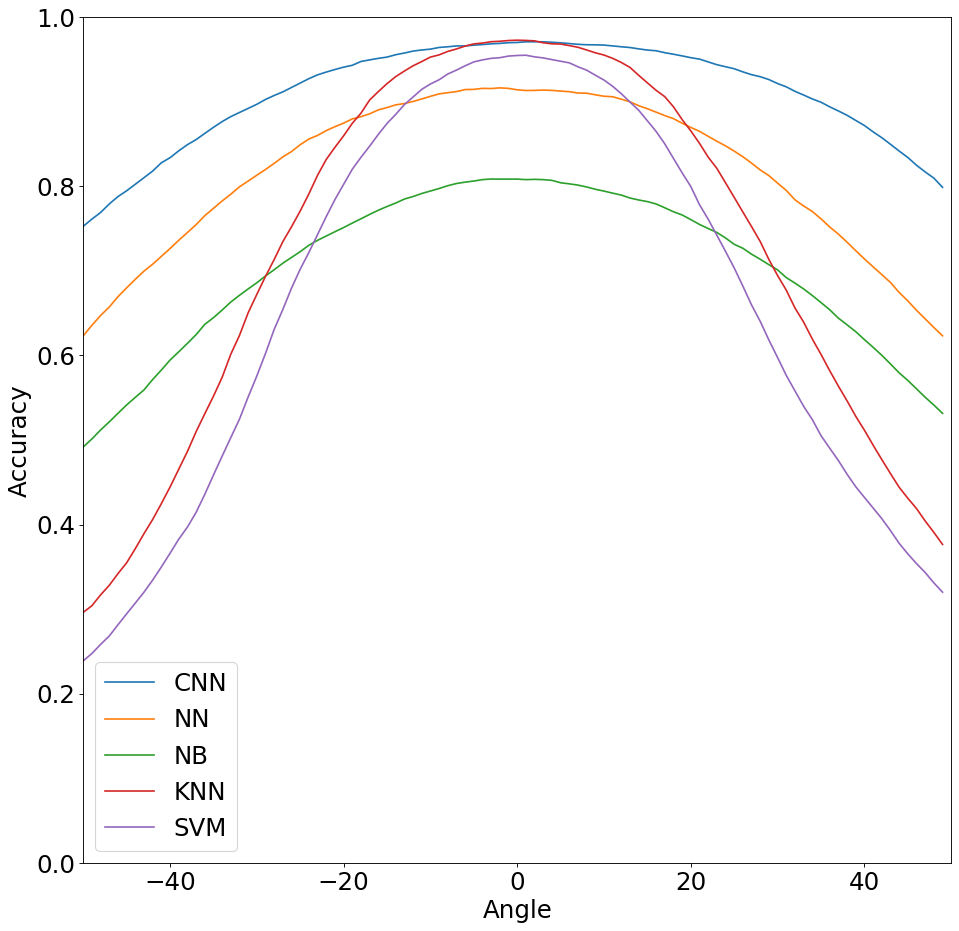
\includegraphics[width=\textwidth]{chapters/results/MT/Rotate.png}
        \caption{Rotation}
    \end{subfigure}
    \begin{subfigure}[b]{ 0.3\textwidth}
        \centering
        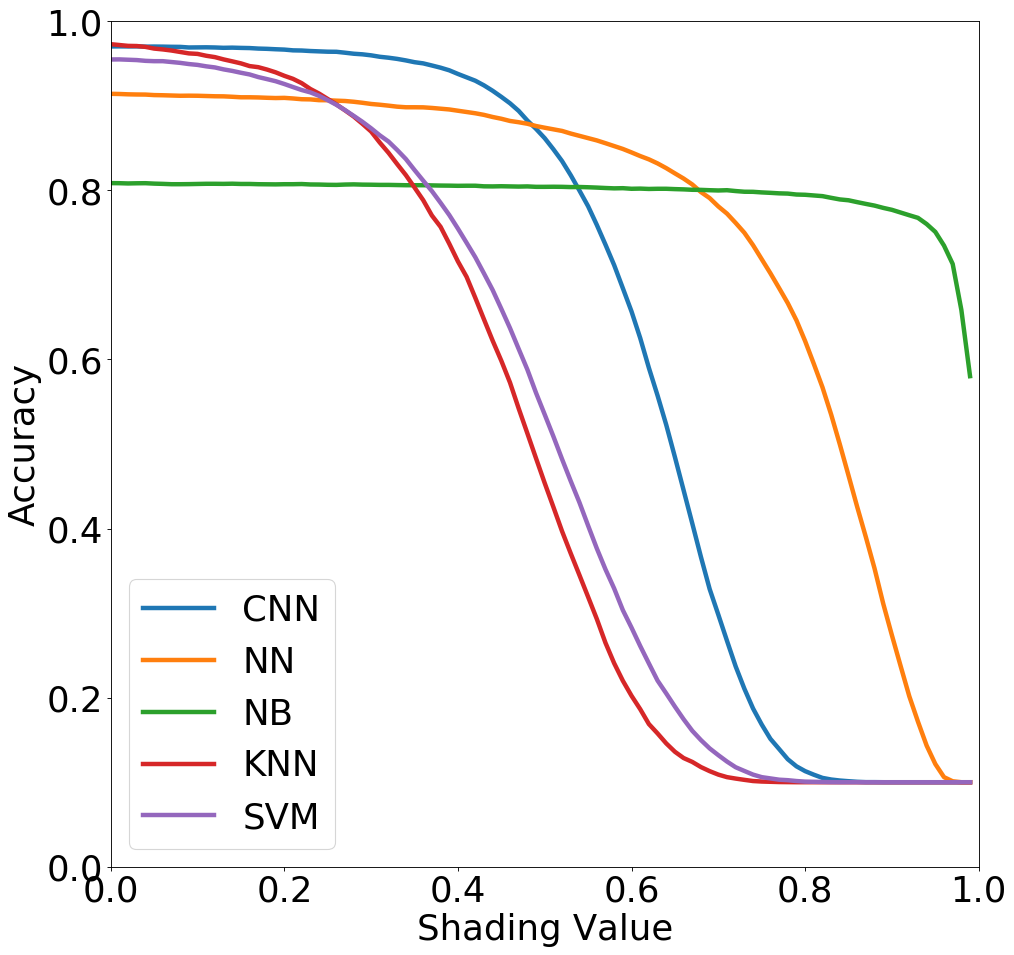
\includegraphics[width=\textwidth]{chapters/results/MT/Shade.png}
        \caption{Shading}
    \end{subfigure}
    \begin{subfigure}[b]{0.3\textwidth}
        \centering
        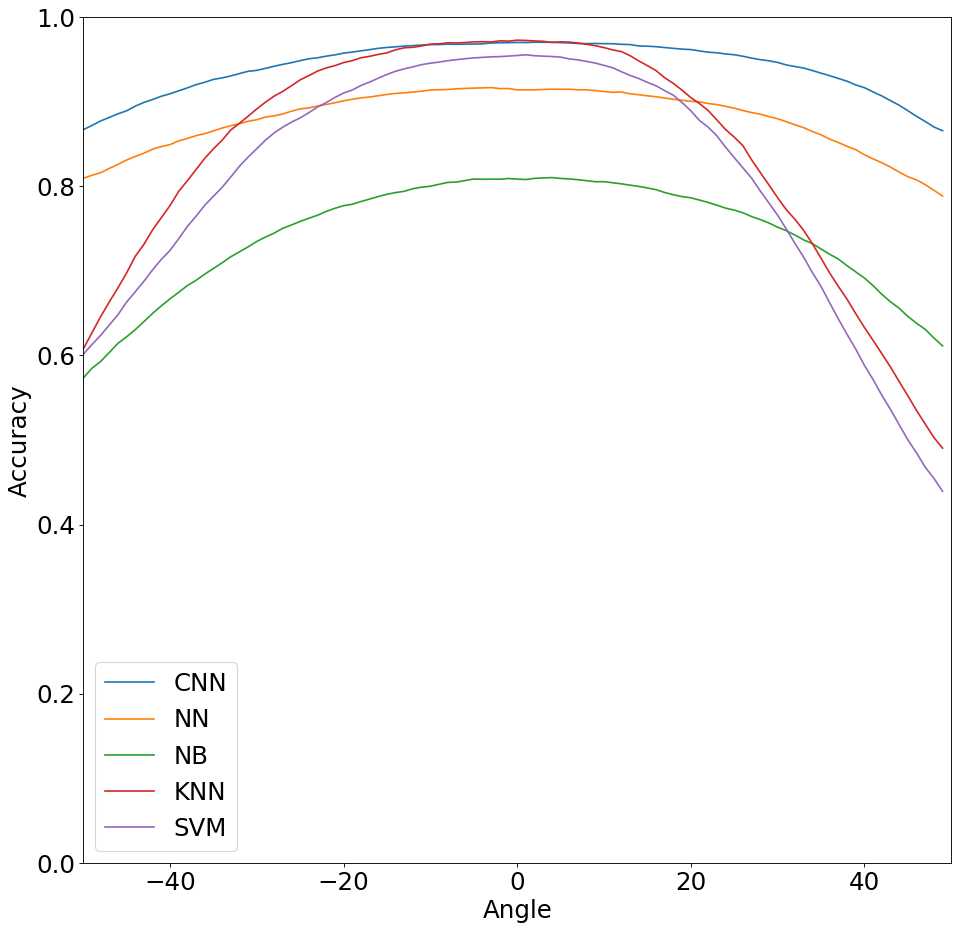
\includegraphics[width=\textwidth]{chapters/results/MT/Shear.png}
        \caption{Shearing}
    \end{subfigure}
    \begin{subfigure}[b]{0.3\textwidth}
        \centering
        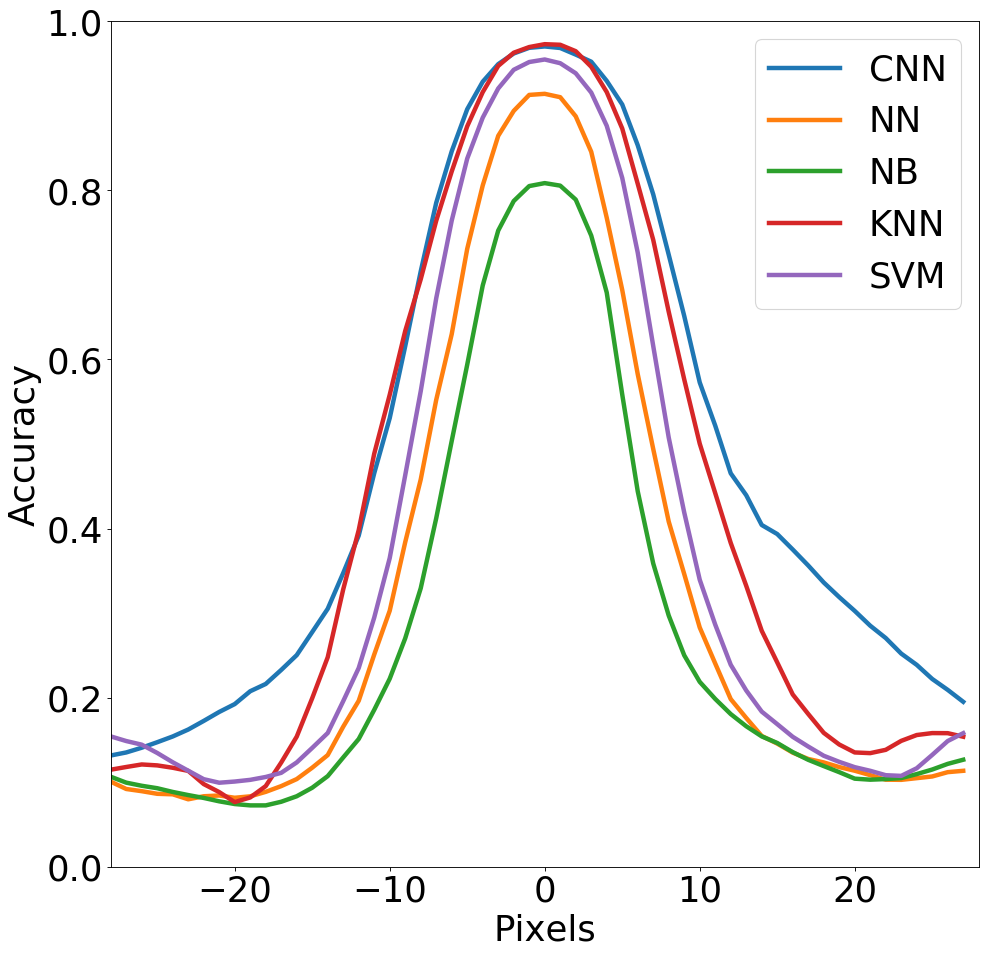
\includegraphics[width=\textwidth]{chapters/results/MT/ShiftX.png}
        \caption{Shifting along X-axis}
    \end{subfigure}
    \begin{subfigure}[b]{0.3\textwidth}
        \centering
        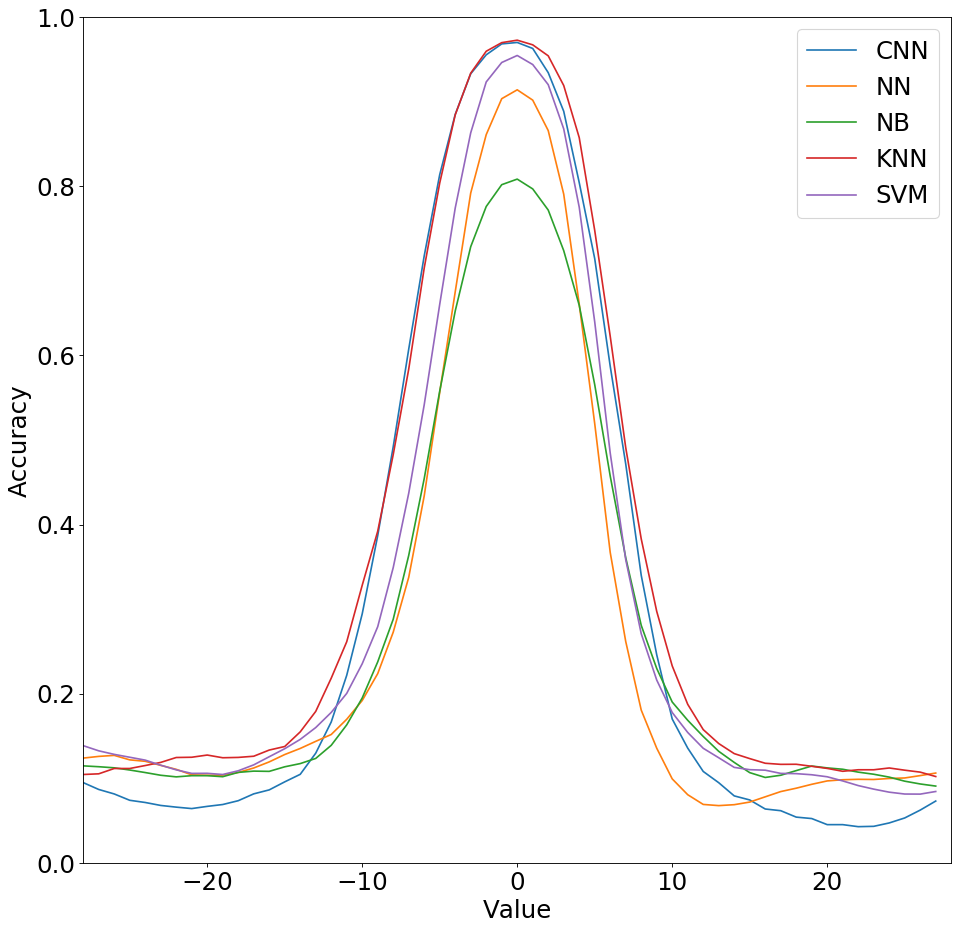
\includegraphics[width=\textwidth]{chapters/results/MT/ShiftY.png}
        \caption{Shifting along Y-axis}
    \end{subfigure}
    \caption{Accuracy of the algorithms.}
    \label{fig:Accuracy}
    \end{figure}

 From the graphs in \ref{fig:Accuracy} we can see that different algorithms respond differently to the follow-up datasets. To quantify this difference, we calculated the area under curve for all the curves in \ref{fig:Accuracy}. The following table shows the area under each curve in \ref{fig:Accuracy}.
    \begin{table}[ht]
    \centering
        \begin{tabular}{|c|c|c|c|c|c|}
        \hline
         & CNN & NN & NB & KNN & SVM \\
         \hline
        Rotation & 91.01 & 81.70 & 70.31 & 72.71 & 66.60  \\
        \hline
        Shading & 64.40 & 75.51 & 79.52 & 50.26 & 52.23 \\
        \hline
        Shearing & 94.07 & 87.95 & 74.23 & 84.26 & 81.08 \\
        \hline
        Shift-X & 48.51 & 32.06 & 27.36 & 42.33 & 36.88 \\
        \hline
        Shift-Y & 30.32 & 26.19 & 26.55 & 34.04 & 29.90 \\
        \hline
        \end{tabular}
        \caption{Area under curve.}
        \label{tbl:test-file-format}
    \end{table}
    Figure 4.1(a) through (c) shows the variation in accuracy of . A higher area under curve means 
    KNN has a higher accuracy but, the area under curve is much lower than the convolutional neural network and the 2-layer neural network. Suggests that if you want to use metamorphic transformation to reveal flaw in an algorithm some transformations may be preferable over others.
    

\subsection{Class Accuracy}\label{Digit-by Accuracy}
    We discussed several papers in Section \ref{2.4MetamorphicTestingMachineLearning} on how the metamorphic relations affect datasets but none of them have investigated how the transformations affect the individual classes in those dataset. It is trivially easy to imagine that not all the data points in a dataset will be affected in the same way with all the transformations. For example, the digit $0$ will still be easily recognizable as $0$ even if it is rotated by 180\textdegree  due to it's symmetry. On the other hand, the digit $9$ can easily be confused with digit $6$ if rotated clockwise by 180\textdegree and vice-versa. Due to this non-uniform affect of transformations on the different data points we decided to investigate how each class of data points affects the accuracy of the model. Thus, besides studying the overall effect of the metamorphic transformations on the whole dataset, we will also study how they affect individual data classes in the MNIST dataset. 
    
    Figure 4.2 to 4.7 shows the accuracy of MNIST dataset class labels $[0-9]$ for our metamorphic relations. Every figure in Figure 4.2-4.7 has ten sub-graphs, each, representing the correct classification of a class label. We want to see if there was a major difference in how each class is affected by a metamorphic relation to get a sense for robustness of the whole dataset. To quantify this we calculated the area under curve for each of the sub-graphs in tables \ref{tbl:test-file-formatRotate}-\ref{tbl:test-file-formatShiftY}. A higher area under curve means that the class was less influenced by the transformation with respect to other classes and it's accuracy on the transformed testing input will be closer to training data.
    
    Figure \ref{fig:Digit by misclassification for Rotation MR} shows the graphs for the accuracy of the classes in the MNIST dataset after applying the rotation transformation. There are five subplots in each sub-graph in Figure \ref{fig:Digit by misclassification for Rotation MR}. Each subplot represents the accuracy of that digit for the five machine learning algorithms we implemented. The X-axis represents the angle with which the test data points were rotated and the Y-axis represents the accuracy of all the test data points in that class.\\
    \begin{figure}[H]
    \centering
        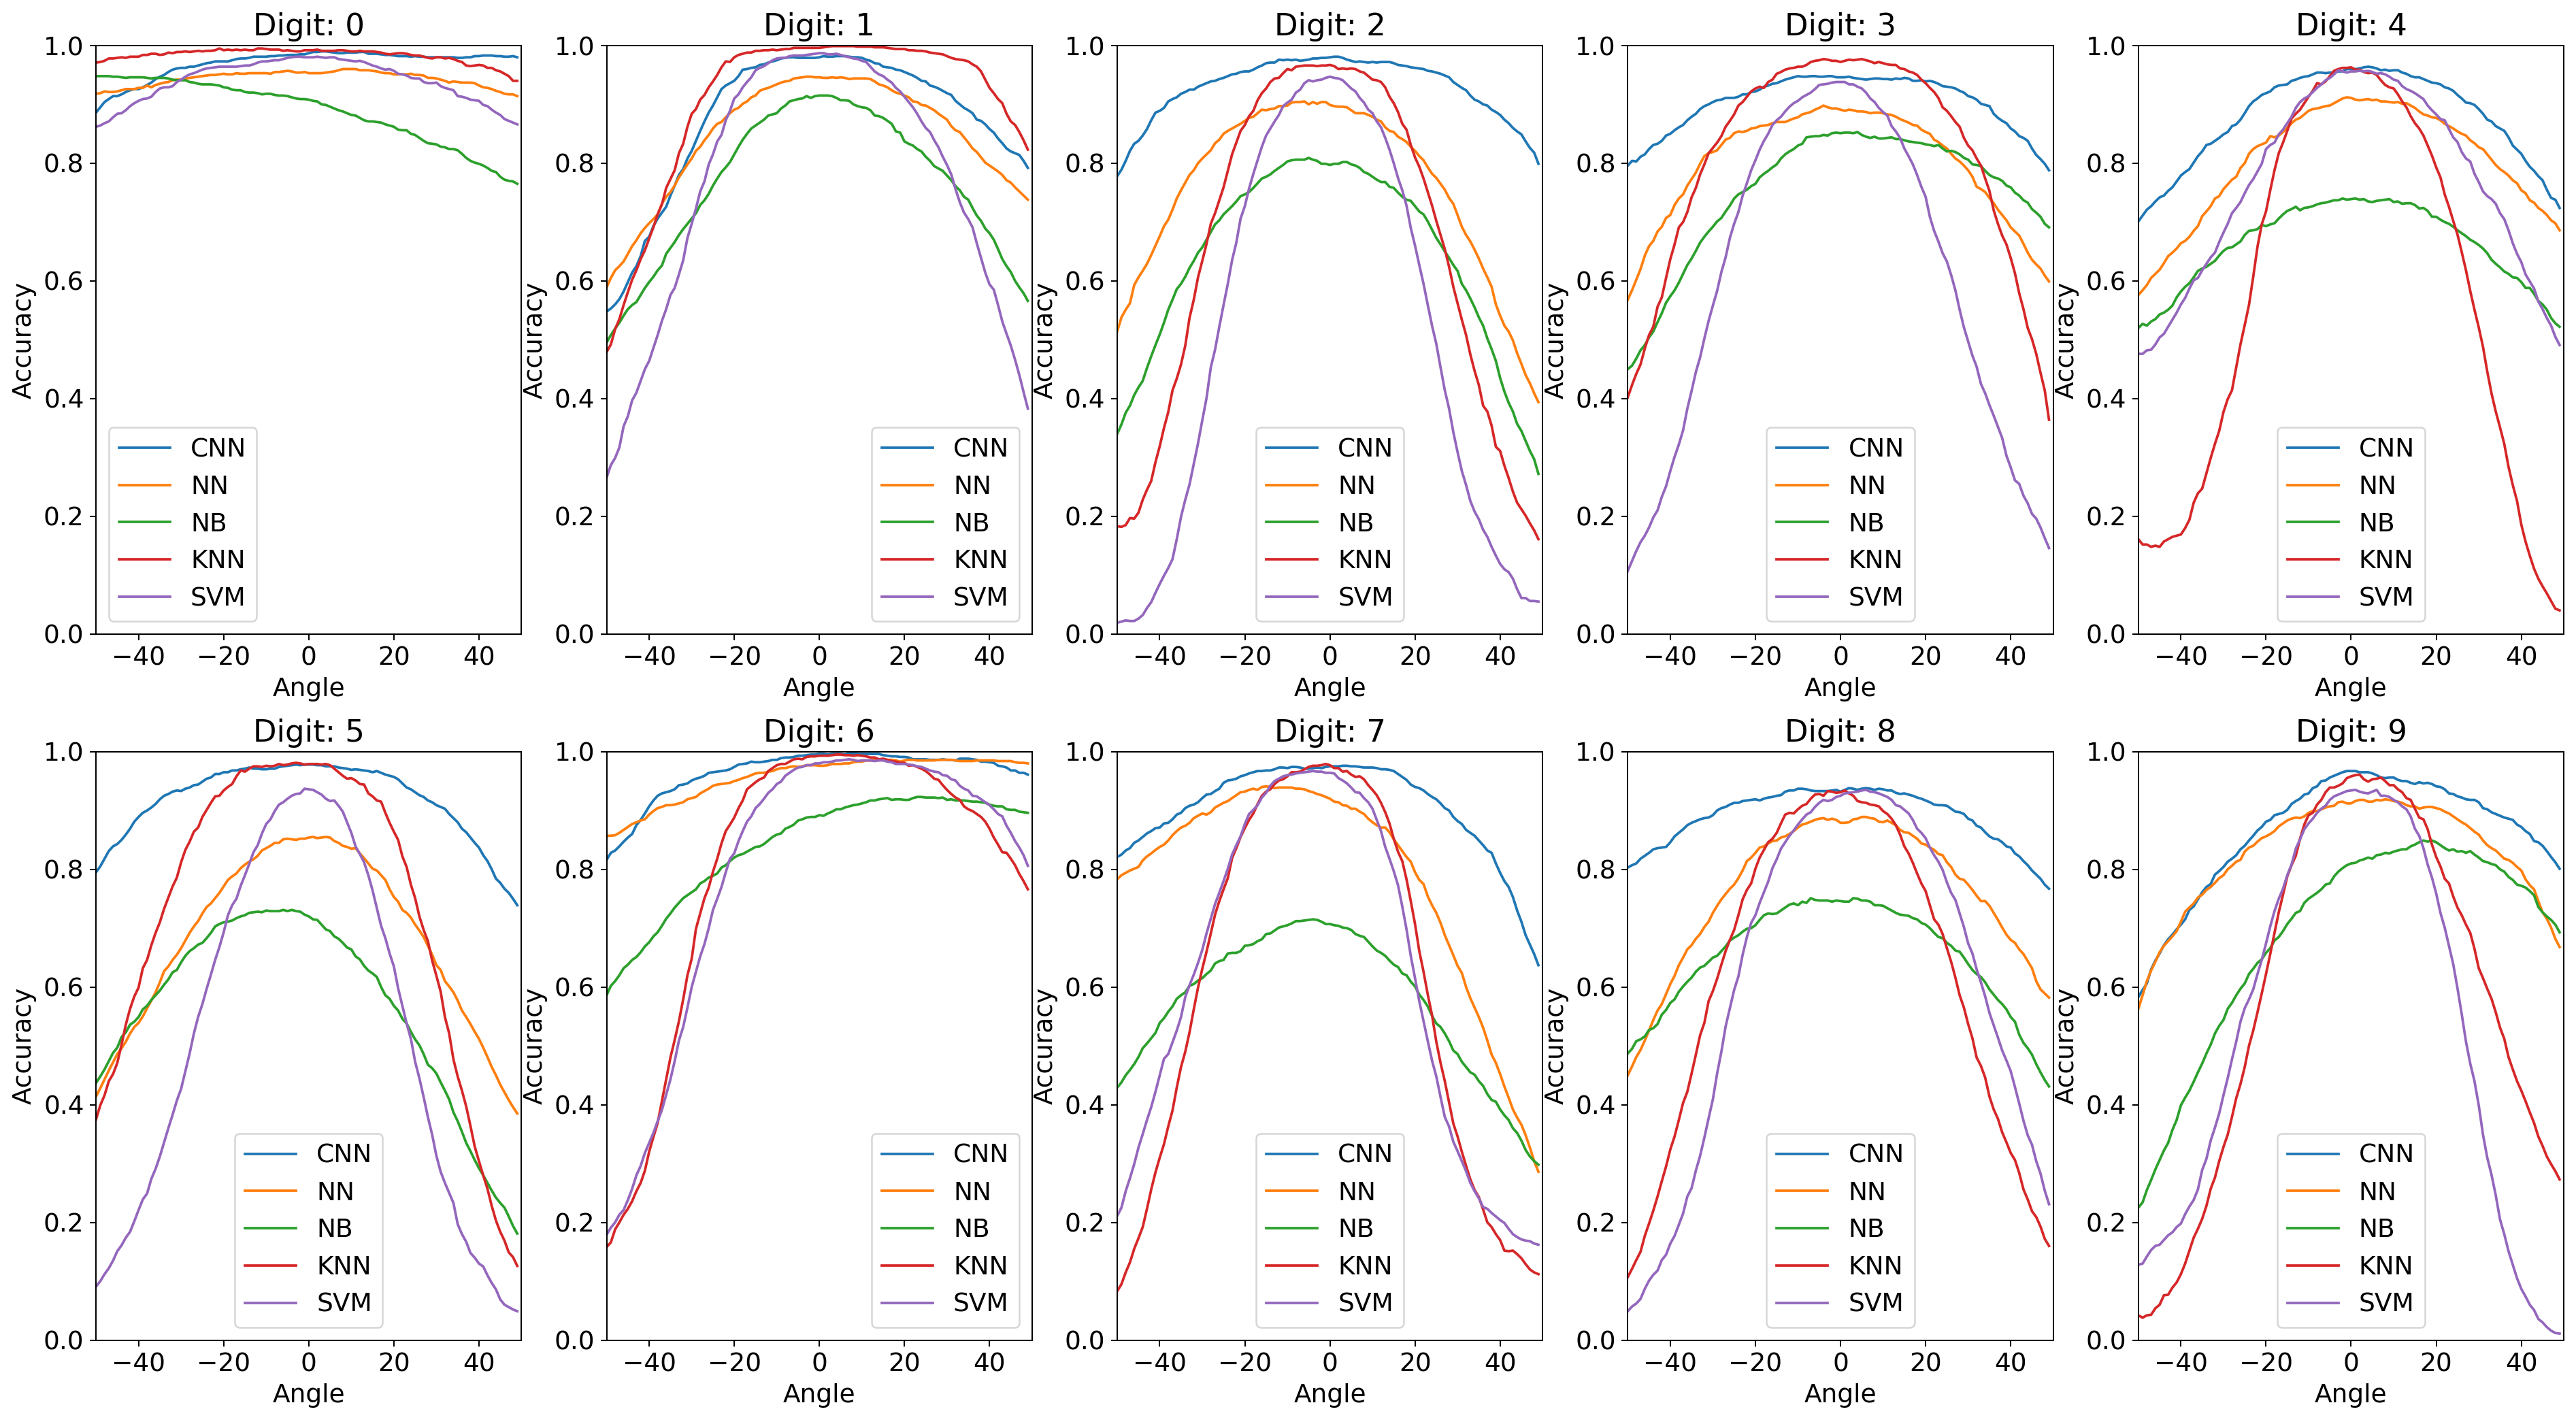
\includegraphics[width=\textwidth]{chapters/results/MT/RotateAll.png}
        \caption{Class accuracy for MT:Rotate}
        \label{fig:Digit by misclassification for Rotation MR}
    \end{figure}
    
    We did similar analysis for all the metamorphic property we identified in section \ref{identifyingMR}. For every class in the MNIST test dataset we applied the transformations with increasing value and calculated the accuracy of the algorithms at each value.\\
    Figure \ref{fig:Digit by misclassification for Shading MR} shows the graphs for the accuracy of each class in MNIST dataset for the shading transformation. The five subplots in each sub-graph in Figure \ref{fig:Digit by misclassification for Shading MR} represents the accuracy of that digit for the five machine learning algorithms we implemented. The X-axis represents the value with which the test data points were shaded and the Y-axis represent the accuracy of all the test data points in that class. We also observed that all the algorithms started to predict the test data points as $1$ once the foreground became dark which is reflected in higher values of accuracy for digit $1$. \\
        
    \begin{figure}[ht!]
    \centering
        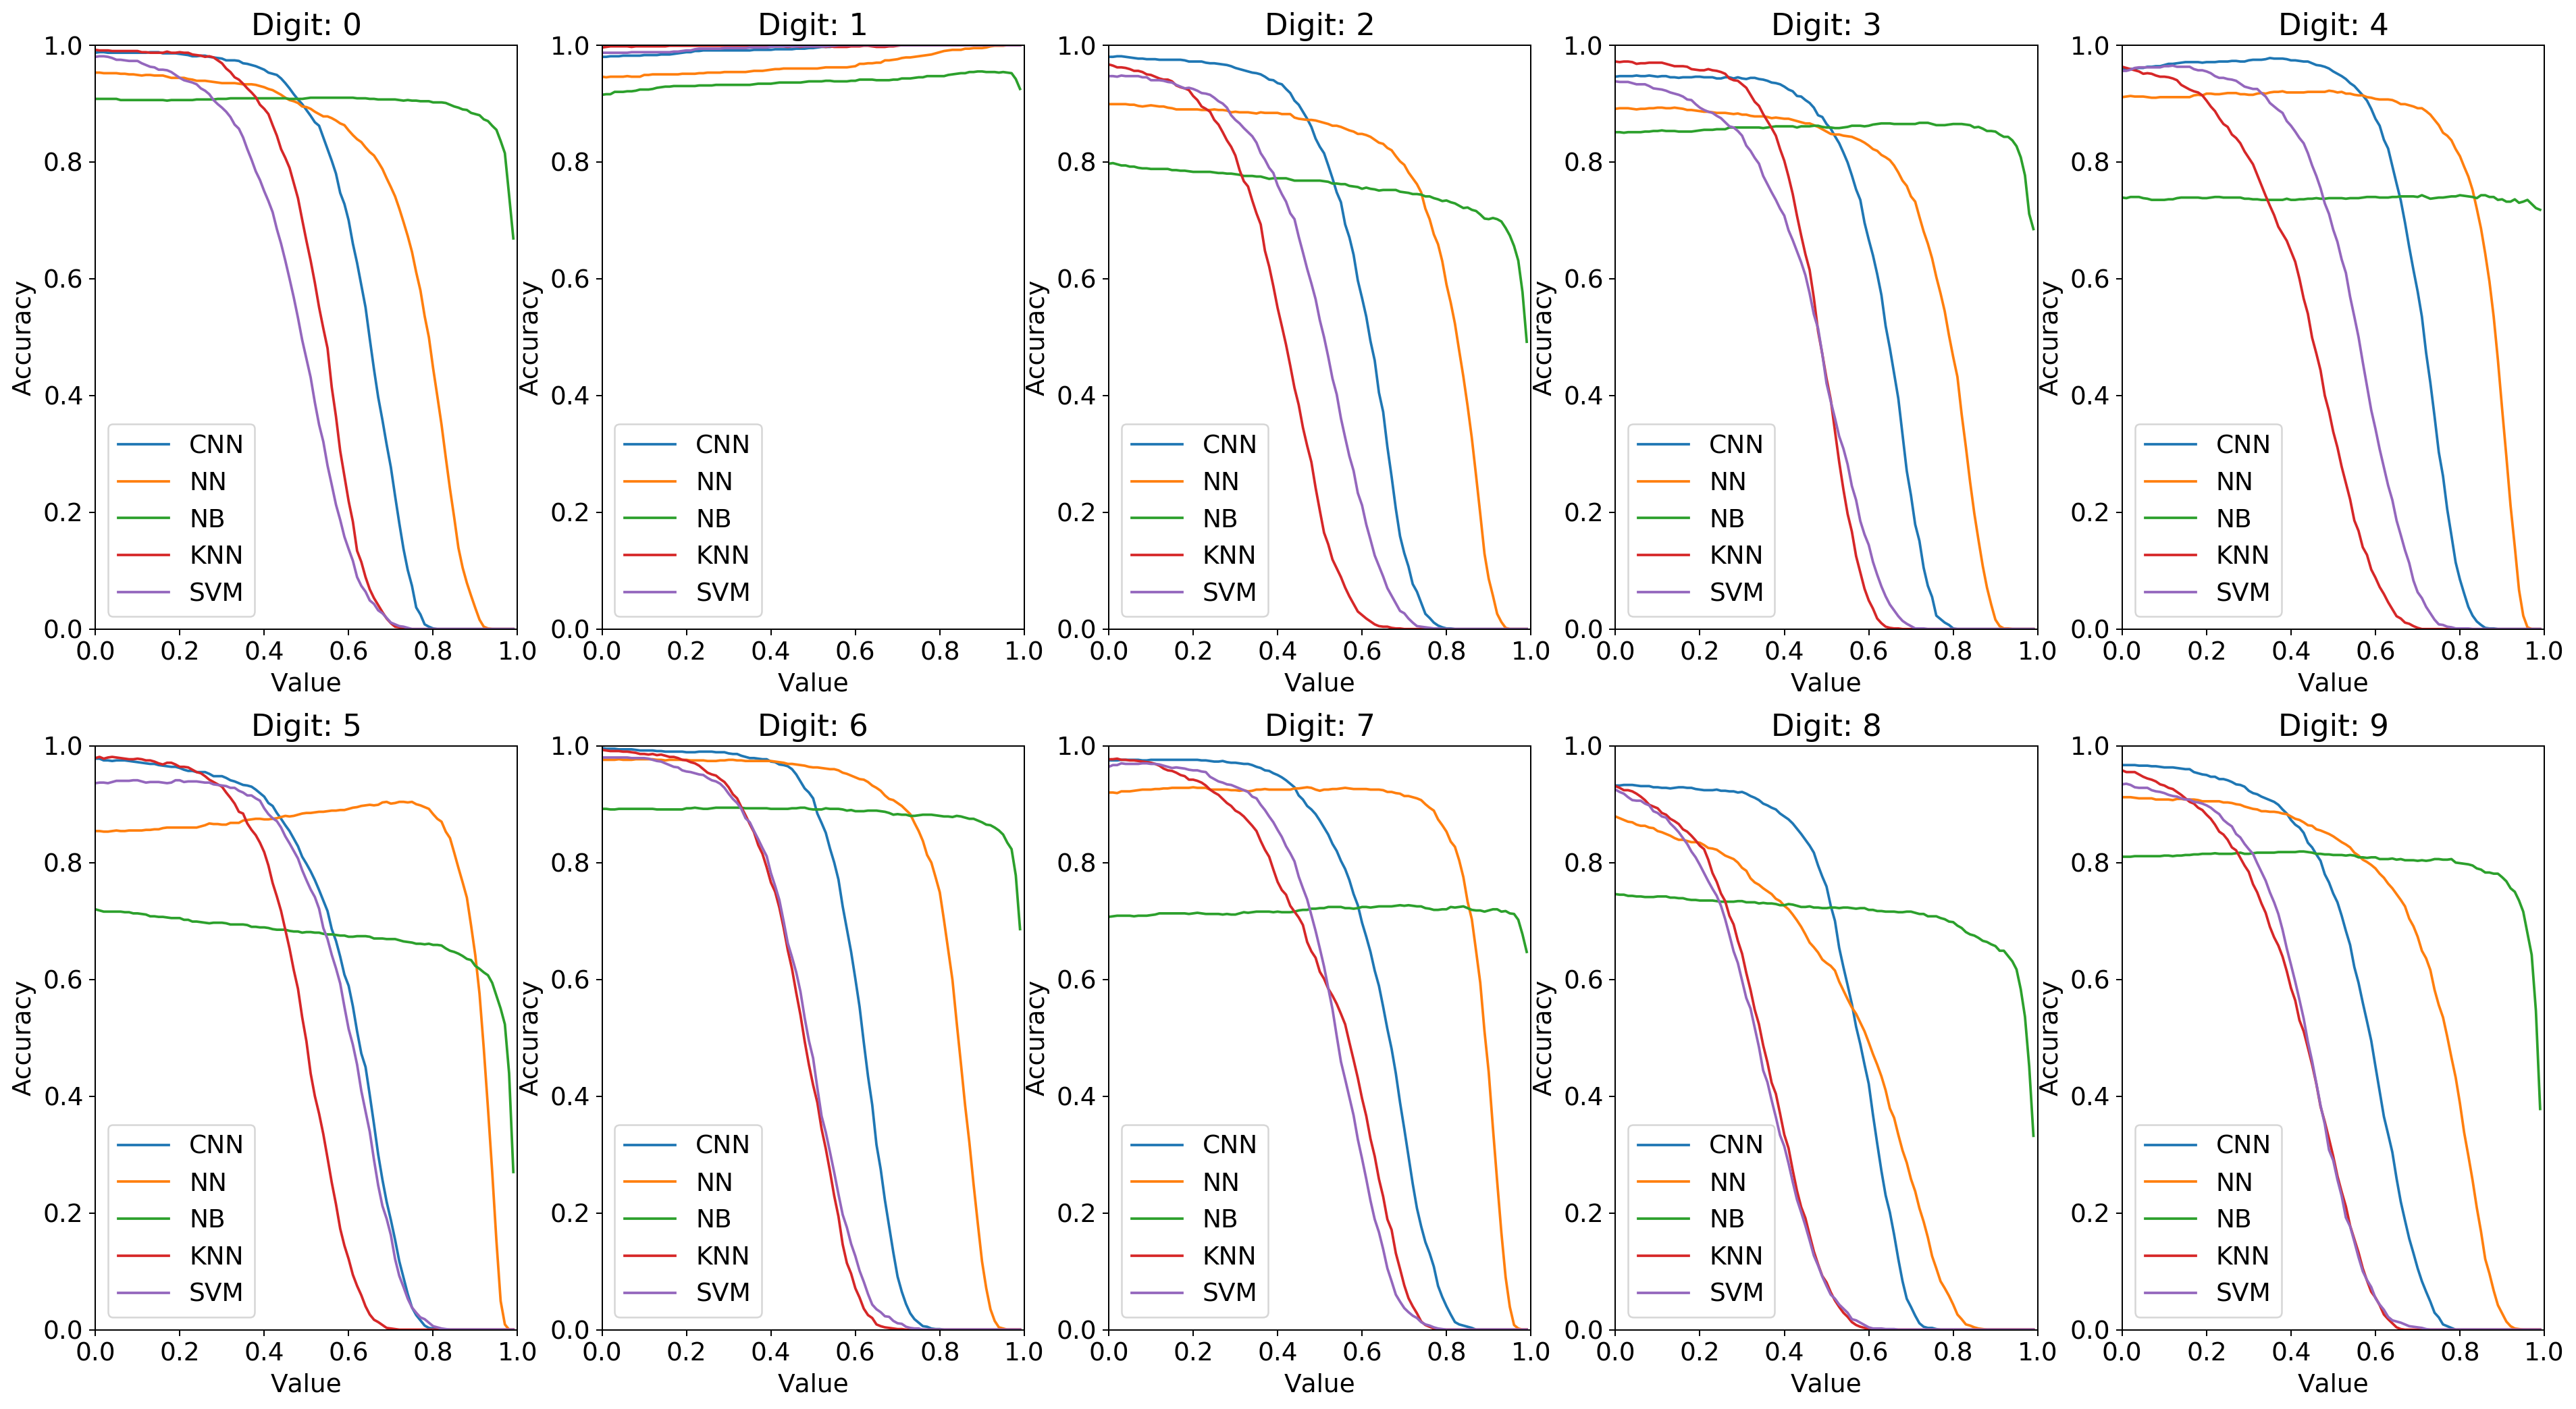
\includegraphics[width=\textwidth]{chapters/results/MT/ShadeAll.png}
        \caption{Class accuracy for MT:Shading}
        \label{fig:Digit by misclassification for Shading MR}
    \end{figure}
    
    The following graphs shows similar graphs for the metamorphic properties shear, shifting the images on X axis, shifting the images on Y axis.
    
    \begin{figure}[H]
    \centering
        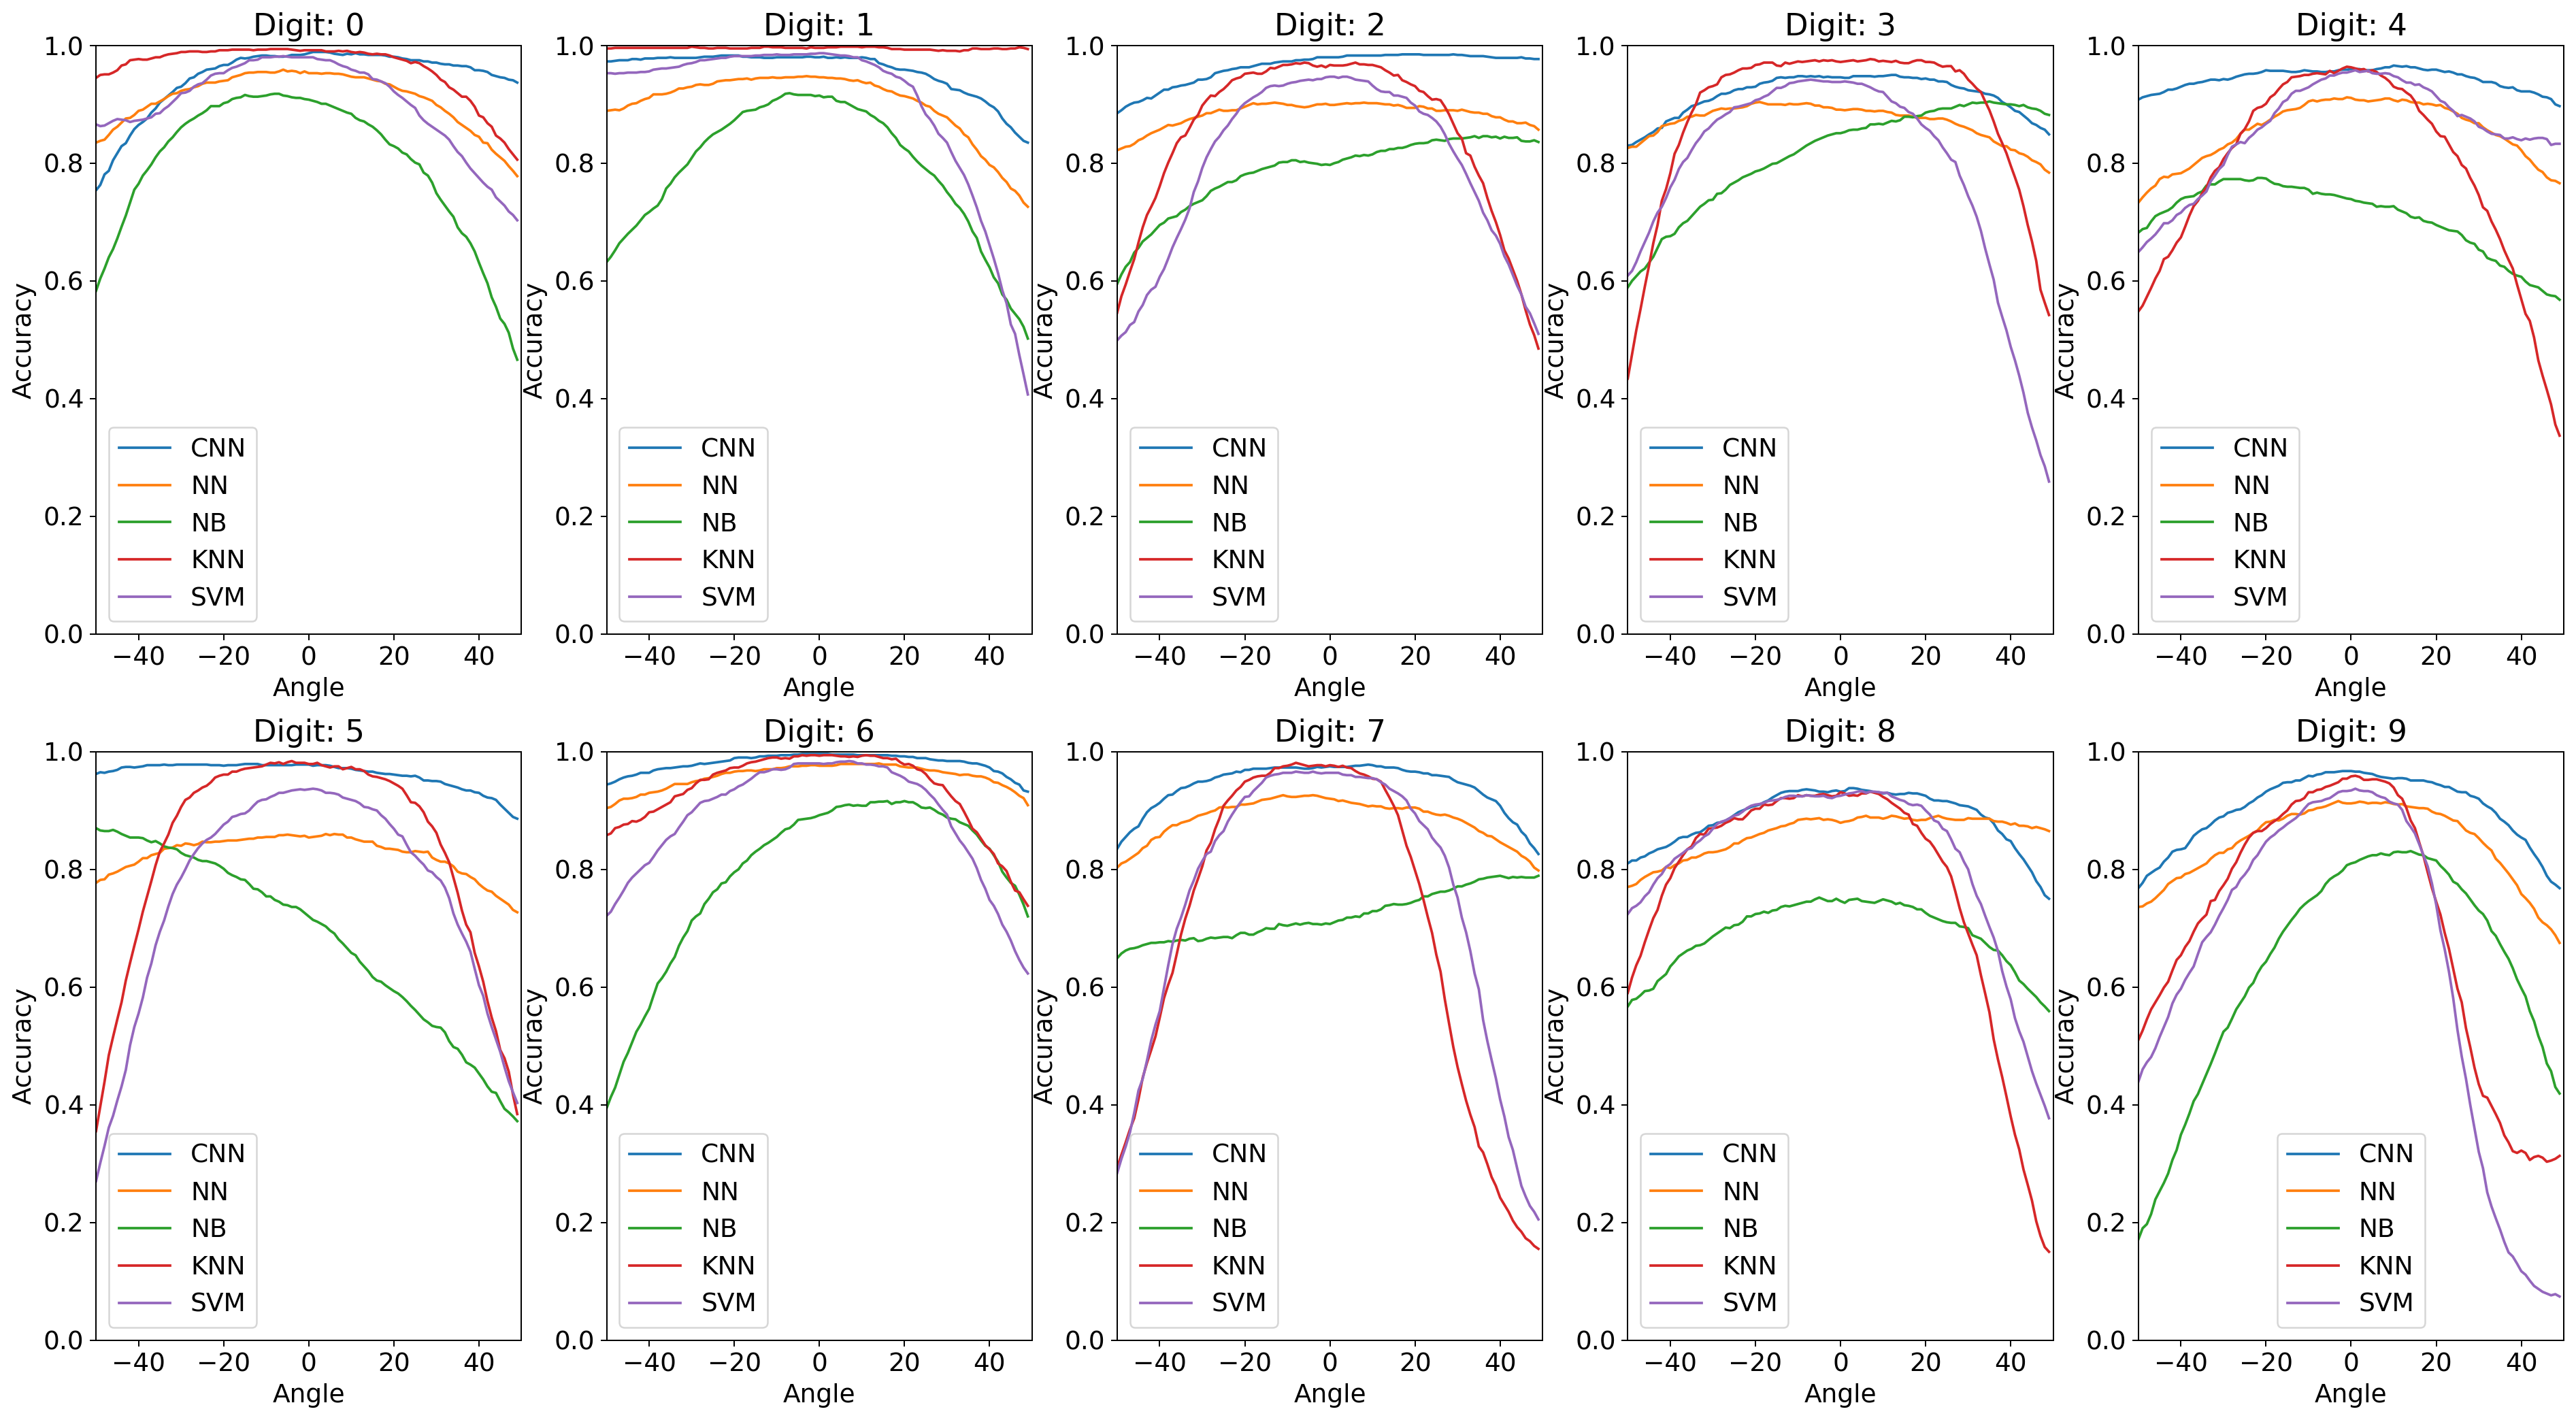
\includegraphics[width=\textwidth]{chapters/results/MT/ShearAll.png}
        \caption{Class accuracy for MT:Shear}
        \label{fig:Digit by misclassification for Shear MR}
    \end{figure}
    
    \begin{figure}[ht!]
    \centering
        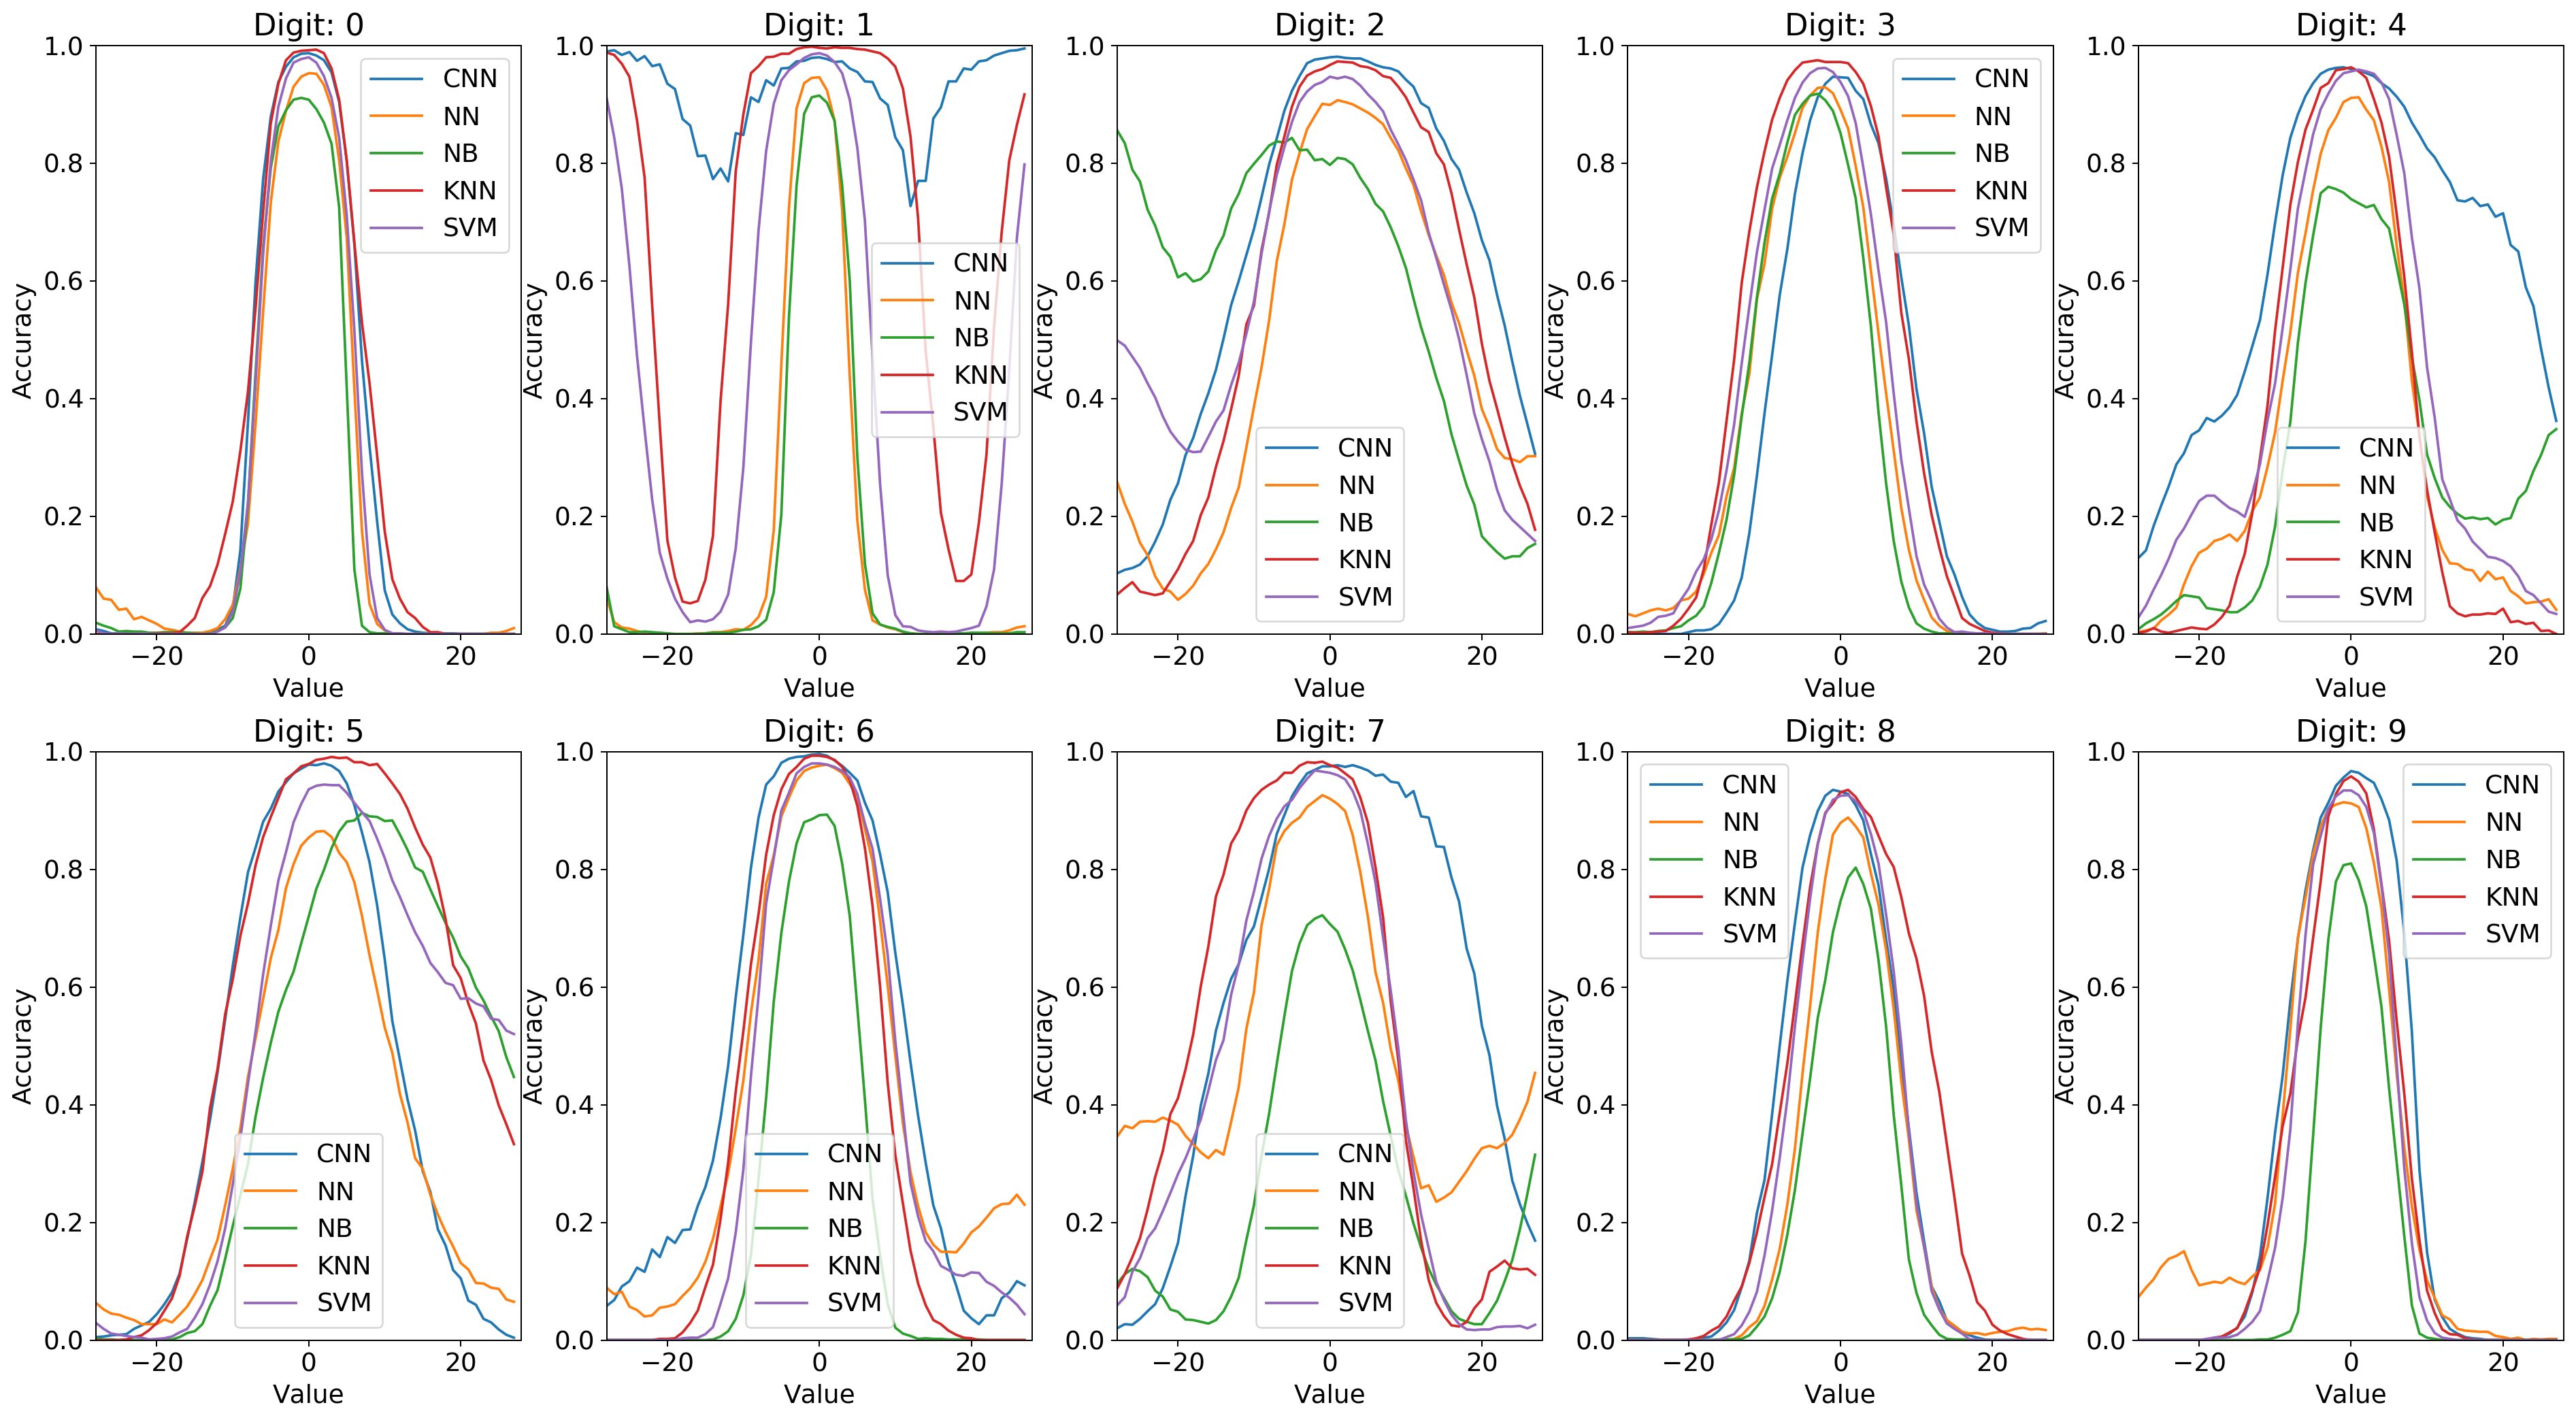
\includegraphics[width=\textwidth]{chapters/results/MT/ShiftXAll.png}
        \caption{Class accuracy for MT: ShiftX}
        \label{fig:Rotate-misclass0}
    \end{figure}
    
    \begin{figure}[H]
    \centering
        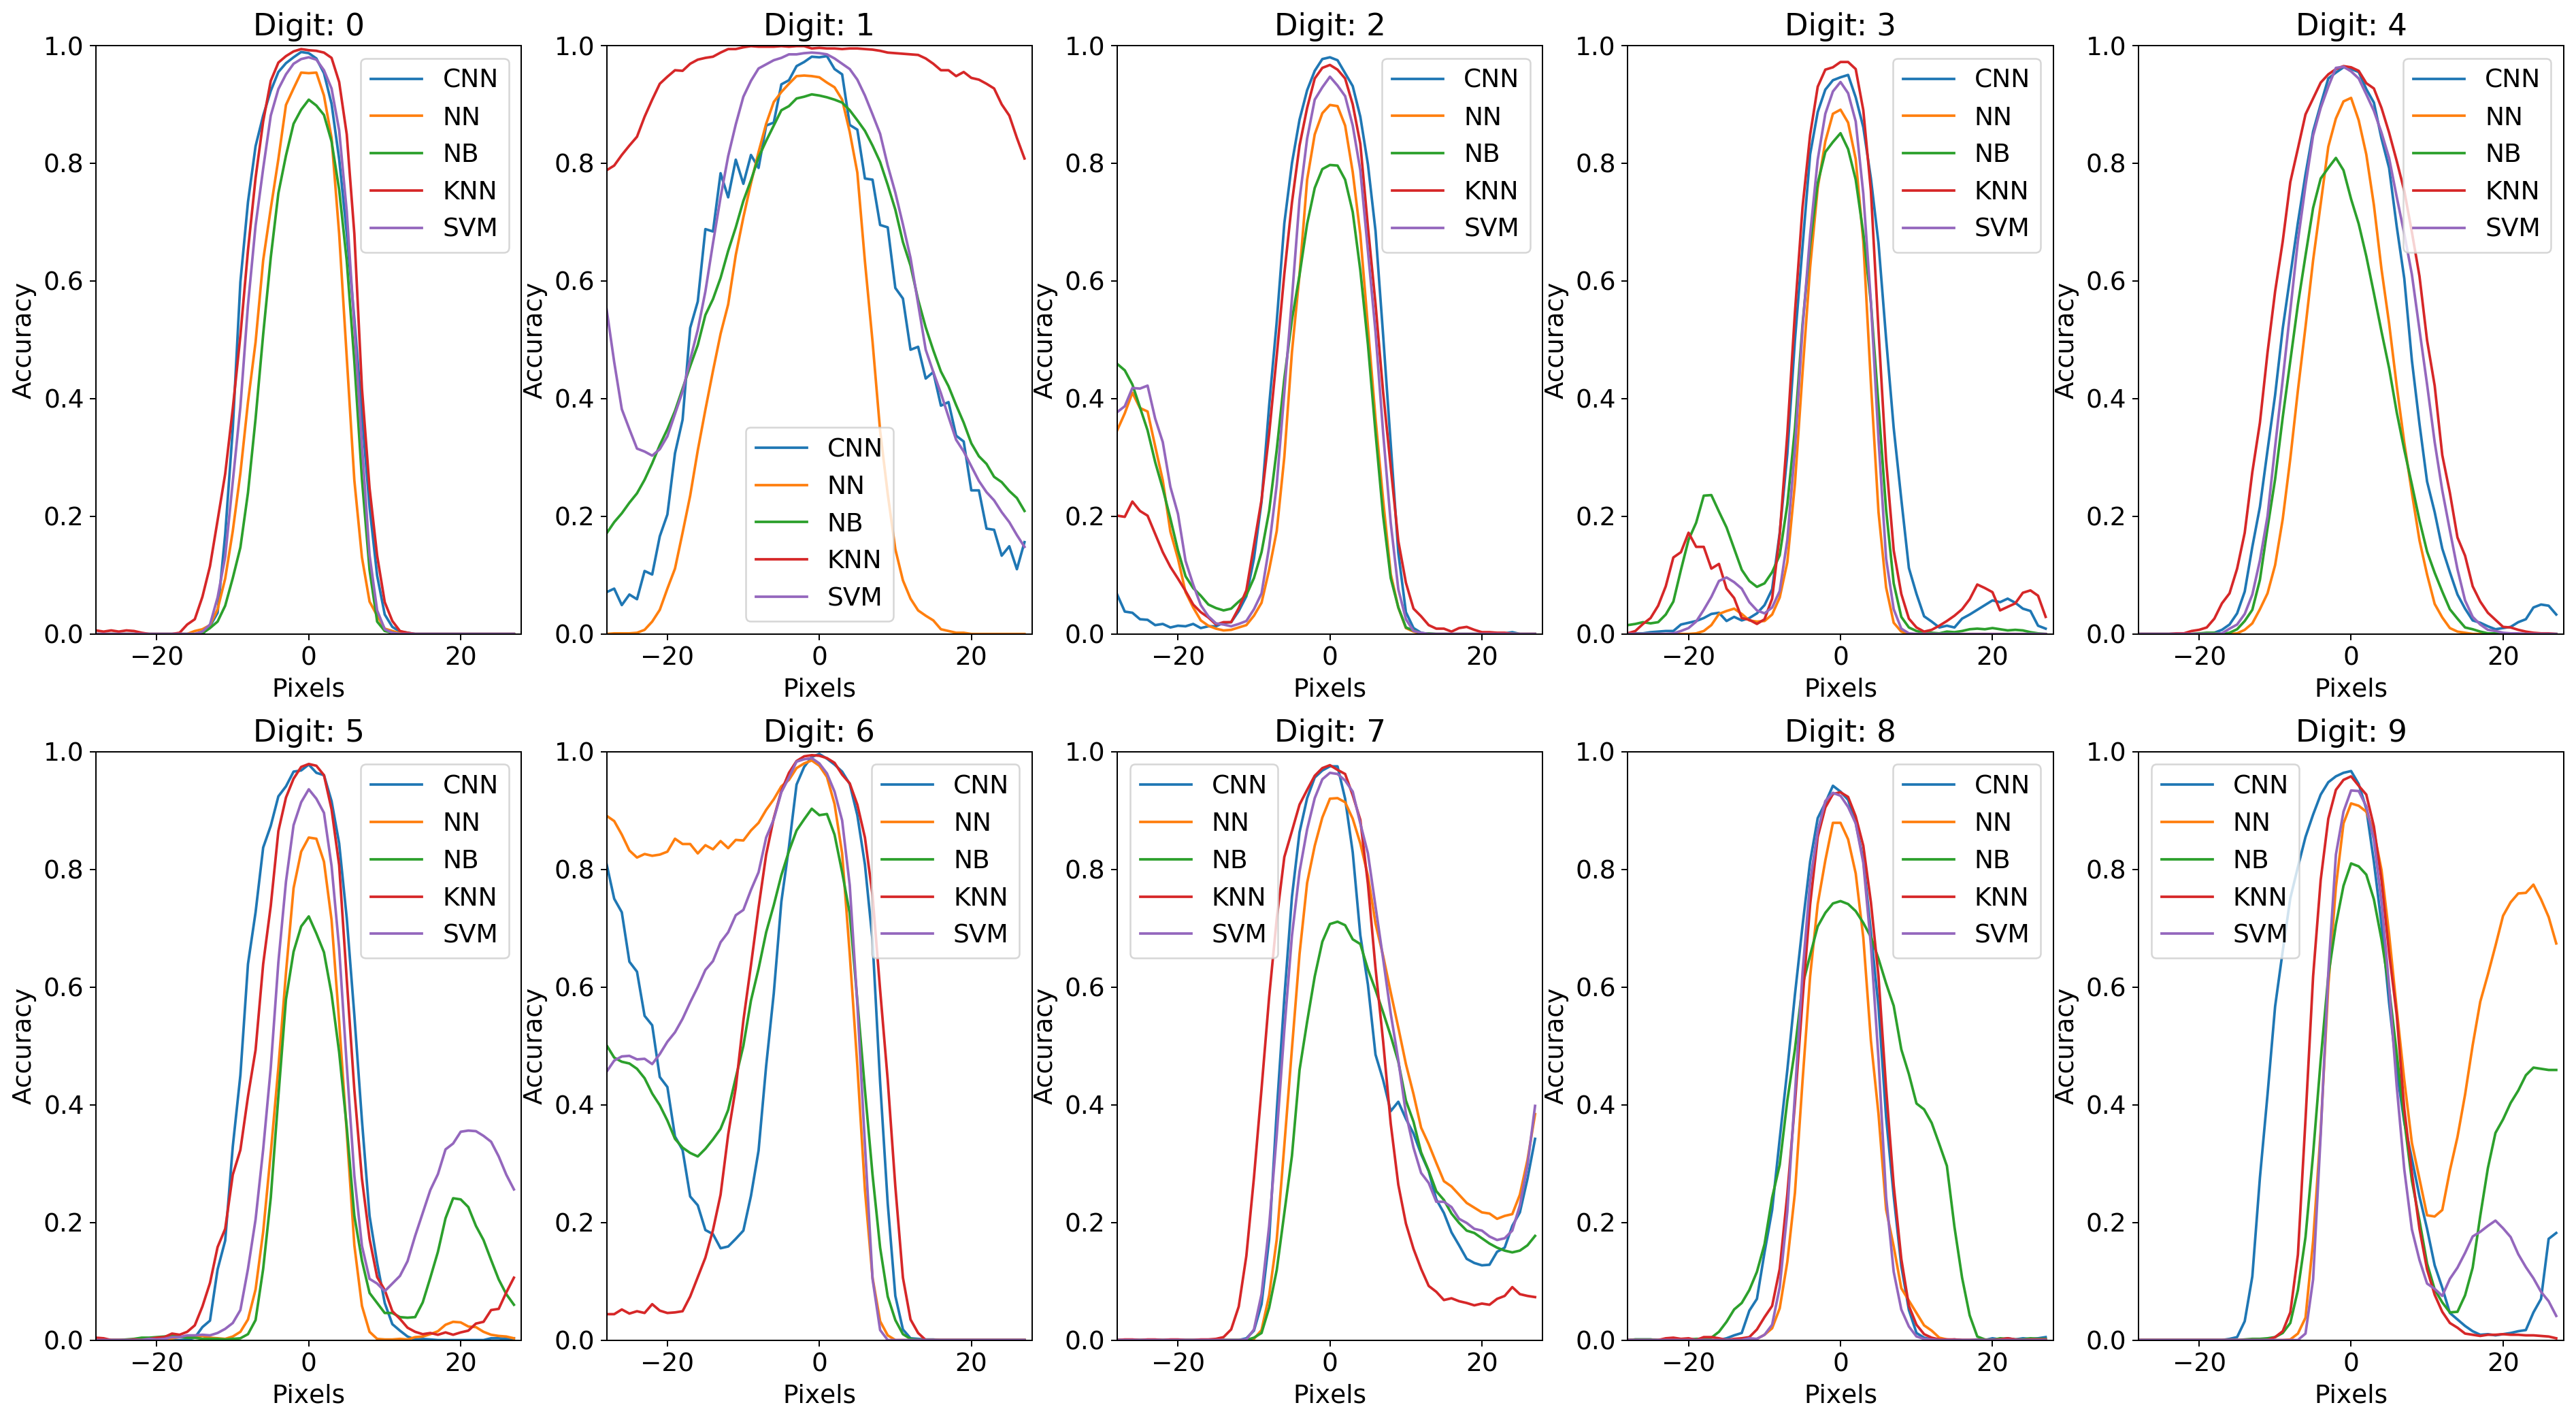
\includegraphics[width=\textwidth]{chapters/results/MT/ShiftYAll.png}
        \caption{Class accuracy for MT: ShiftY}
        \label{fig:Rotate-misclass0}
    \end{figure}
    
    To further compare the accuracy of the different classes we calculated the area under each curve. The following tables shows the area under curve for each class $[0,9]$ in the above graphs. The cells with \textcolor{green}{green} background has the highest value among all the cells in that row and the ones in \textcolor{red}{red} has the lowest.
    \begin{table}[H]
    \centering
        \begin{tabular}{|c|c|c|c|c|c|c|c|c|c|c|}
        \hline
         & 0 & 1 & 2 & 3 & 4 & 5 & 6 & 7 & 8 & 9 \\
        \hline
        CNN & \cellcolor{green!25} 97.01 & 87.69 & 92.87 & 90.29 & 87.77 & 91.86 & 96.54 & 90.47 & 88.99 & \cellcolor{red!25}86.62 \\ 
        \hline
        NN &   94.34 & 84.75 & 75.98 & 79.87 & 80.47 & \cellcolor{red!25}68.33 & \cellcolor{green!25}95.66 & 78.64 & 76.16 & 82.76 \\
        \hline
        NB & \cellcolor{green!25}88.80 & 76.64 & 64.08 & 75.23 & 66.16 & \cellcolor{red!25}56.60 & 84.09 & 57.65 & 65.20 & 68.69 \\
        \hline
        KNN & \cellcolor{green!25}98.31 & 90.80 & 65.39 & 81.12 & \cellcolor{red!25}56.70 & 73.24 & 80.56 & 60.03 & 62.05 & 58.92 \\
        \hline
        SVM & \cellcolor{green!25}93.97 & 76.54 & \cellcolor{red!25}50.38 & 60.45 & 76.49 & 51.74 & 79.87 & 61.49 & 61.58 & 53.49 \\
        \hline
        \end{tabular}
        \caption{Area under curve for each class for MR: Rotation.}
        \label{tbl:test-file-formatRotate}
    \end{table}
    
     From the table \ref{tbl:test-file-formatRotate} we can see that the digit $0$ has the highest area under curve in the convolutional neural network implementation and the digit $9$ has the lowest area. From this we can say that the accuracy of the sub-set of MNIST dataset with class label $0$ is not affected as much as the other classes when the rotation property is applied. Thus, when creating follow-up test cases for a convolutional neural network, the tester can apply the rotation property to the digit $0$ to a larger angle than any other classes. We will make these recommendations more concrete in \ref{tbl:indexrecommendations}.\\
     We generated the following tables to perform the same analysis on all the metamorphic properties. The digits with red background have the lowest area under curve for that algorithm thus, the lowest average accuracy for all the degree of transformation. The cells with green background have the highest area under curve and thus the highest average accuracy for all the degree of transformation. 
    
    \begin{table}[H]
    \centering
    \begin{tabular}{|c|c|c|c|c|c|c|c|c|c|c|c|}
    \hline
     & 0 & 1 & 2 & 3 & 4 & 5 & 6 & 7 & 8 & 9 \\
    \hline
    CNN & 63.02 & \cellcolor{green!25}99.38 & 59.26 & 60.58 & 69.07 & 58.96 & 60.93 & 63.65 & \cellcolor{red!25}53.64 & 55.51 \\ 
    \hline
    NN & 72.64 & \cellcolor{green!25}96.66 & 72.61 & 69.35 & 80.50 & 80.77 & 81.16 & 82.36 & \cellcolor{red!25}50.98 & 68.08 \\
    \hline
    NB & 89.85 & \cellcolor{green!25}93.71 & 75.36 & 85.34 & 73.75 & \cellcolor{red!25}67.04 & 88.28 & 71.61 & 70.71 & 79.58 \\
    \hline
    KNN & 52.81 & \cellcolor{green!25}99.87 & 39.91 & 46.68 & 42.49 & 48.36 & 47.00 & 52.17 & \cellcolor{red!25}32.81 & 40.52 \\
    \hline
    SVM & 47.12 & \cellcolor{green!25}99.61 & 47.91 & 44.62 & 53.40 & 56.73 & 47.62 & 52.26 & \cellcolor{red!25}31.80 & 41.23 \\
    \hline
    \end{tabular}
    \caption{Area under curve for each class for MR: Shading.}
    \label{tbl:test-file-formatShade}
    \end{table}
    From the table \ref{tbl:test-file-formatShade} we can see that the digit $1$ had the highest accuracy as compared to other classes in the dataset for every algorithm we implemented. On the other hand, the digit $8$ had the lowest accuracy in four out of the five algorithms we implemented.
    Digit $6$ has the highest area under curve in the CNN and NN algorithms. The digits $3$, $1$, and, $0$ have the highest area under curve in the NB, KNN, and, SVM implementations respectively.
    
    \begin{table}[H]
    \centering
    \begin{tabular}{|c|c|c|c|c|c|c|c|c|c|c|}
    \hline
    & 0 & 1 & 2 & 3 & 4 & 5 & 6 & 7 & 8 & 9 \\
    \hline
    CNN & 94.75 & 95.80 & 96.42 & 91.66 & 94.39 & 96.26 &\cellcolor{green!25}98.05 & 94.18 & \cellcolor{red!25}88.89 & 90.28  \\ 
    \hline
    NN & 90.99 & 90.21 & 88.38 & 87.06 & 85.43 & \cellcolor{red!25}82.57 & \cellcolor{green!25}95.77 & 88.55 & 86.13 & 84.41 \\
    \hline
    NB & 79.97 & 79.09 & 78.67 & \cellcolor{green!25}81.60 & 70.81 & 68.39 & 79.37 & 72.12 & 69.02 & \cellcolor{red!25}63.31 \\
    \hline
    KNN & 96.32 & \cellcolor{green!25}99.54 & 85.20 & 88.43 & 78.91 & 83.46 & 93.39 & \cellcolor{red!25}69.79 & 76.79 & 70.73 \\
    \hline
    SVM & \cellcolor{green!25}90.17 & 90.03 & 79.92 & 78.93 & 85.78 & 76.11 & 88.71 & 75.08 & 82.16 & \cellcolor{red!25}63.90 \\
    \hline
    \end{tabular}
    \caption{Area under curve for each class for MR: Shear.}
    \label{tbl:test-file-formatShear}
    \end{table}
    The digit $6$ has the highest area under curve for CNN and NN while the digits $8$ and $5$ have the lowest area under curve.
    
    \begin{table}[htb!]
    \centering
    \begin{tabular}{|c|c|c|c|c|c|c|c|c|c|c|}
    \hline
    & 0 & 1 & 2 & 3 & 4 & 5 & 6 & 7 & 8 & 9 \\
    \hline
    CNN & \cellcolor{red!25}25.17 & \cellcolor{green!25}92.04 & 65.01 & 31.49 & 64.78 & 42.84 & 46.12 & 61.14 & 27.62 & 28.84 \\
    \hline
    NN & 21.30 & \cellcolor{red!25}15.45 & 48.59 & 30.03 & 31.99 & 33.89 & 40.76 & \cellcolor{green!25}49.62 & 21.58 & 27.42 \\
    \hline
    NB & 19.03 & 14.50 & \cellcolor{green!25}60.03 & 27.11 & 30.67 & 45.91 & 20.14 & 25.42 & 16.63 & \cellcolor{red!25}14.14 \\
    \hline
    KNN & 27.56 & \cellcolor{green!25}67.33 & 56.41 & 39.62 & 32.09 & 58.53 & 34.05 & 50.71 & 32.65 & \cellcolor{red!25}24.31 \\
    \hline
    SVM & \cellcolor{red!25}22.05 & 40.13 & \cellcolor{green!25}57.64 & 33.38 & 39.98 & 49.06 & 35.29 & 43.62 & 24.94 & 22.74 \\
    \hline
    \end{tabular}
    \caption{Area under curve for each class for MR: ShiftX.}
    \label{tbl:test-file-formatShiftX}
    \end{table}
    
    \begin{table}[H]
    \centering
    \begin{tabular}{|c|c|c|c|c|c|c|c|c|c|c|}
    \hline
    & 0 & 1 & 2 & 3 & 4 & 5 & 6 & 7 & 8 & 9 \\
    \hline
    CNN & 26.80 & \cellcolor{green!25}52.91 & 25.32 & 22.45 & 30.47 & 26.39 & 38.99 & 29.25 & \cellcolor{red!25}21.09 & 29.53 \\ 
    \hline
    NN &  20.99 & 35.29 & 22.58 & 14.69 & 20.49 & \cellcolor{red!25}14.18 & \cellcolor{green!25}52.86 & 30.59 & 15.52 & 34.77 \\
    \hline
    NB & 19.95 & \cellcolor{green!25}56.37 & 23.13 & 19.51 & 20.90 & \cellcolor{red!25}16.07 & 36.29 & 23.58 & 24.89 & 24.81 \\
    \hline
    KNN & 28.72 & \cellcolor{green!25}95.26 & 26.83 & 23.77 & 36.41 & 25.06 & 34.64 & 29.50 & \cellcolor{red!25}19.31 & 20.93 \\
    \hline
    SVM & 25.09 & \cellcolor{green!25}61.47 & 26.25 & \cellcolor{red!25}17.09 & 30.53 & 25.75 & 43.48 & 31.59 & 17.84 & 19.90  \\
    \hline
    \end{tabular}
    \caption{Area under curve for each class for MR: ShiftY.}
    \label{tbl:test-file-formatShiftY}
    \end{table}
    
A similar analysis was also done for the Fashion-MNIST, and, EMNIST dataset but due to space limitation they are not reported here, instead, they are reported on the project's github page.

\clearpage
\newpage
In the tables 4.2 to 4.6 we have seen that the different classes are affected differently depending upon the algorithm and the metamorphic transformation applied to them. In this section, we want to make recommendations to pick the best values for the metamorphic properties such that the the accuracy of the transformed dataset will be close to the original dataset. For our purpose we define accuracy being close as within $90\%$ of the origin dataset. To do this we first calculated the accuracy of each class in the original dataset without applying any transformation. We then calculated the degrees of transformation for which the accuracy of the transformed dataset was greater than or equal to $90\%$ of the accuracy of the original dataset for the five algorithms. Based on this exercise we make the recommendation to testers who want to use these properties to generate follow-up test cases. The following table shows the minimum and maximum values of transformations where the accuracy was found to be within $90\%$ of the accuracy without any transformation.

% \pgfplotstableread[row sep=\\,col sep=&]{
%   Class & RotateX & RotateY & ShadeX & ShadeY & ShearX & ShearY & ShiftXx & ShiftXy    & ShiftYx & ShiftYy\\
%     0 &     0 &     35 &         0.1 &     51      & 0.2 & 22    & 0.3        & 3         & 0.4       & 2  \\
%     1 &     200 &     22 &        200.1 &     99      & 200.2 & 20    & 200.3        & -25       & 200.4       & 3  \\
%     2 &     400 &     12 &        400.1 &     50      & 400.2 & 26    & 400.3        & -24       & 400.4      & 2  \\
%     3 &     600 &     13 &        600.1 &     51      & 600.2 & 22    & 600.3        & 1         & 600.4       & 2  \\
%     4 &     800 &     15 &        800.1 &     51      & 800.2 & 19    & 800.3        & 4         & 800.4       & 1  \\
%     5 &     1000 &     10 &        1000.1 &     50      & 1000.2 & 11    & 1000.3        & 6         & 1000.4       & 2  \\
%     6 &     1200 &     37 &        1200.1 &     50      & 1200.2 & 30    & 1200.3        & 3         & 1200.4       & -27  \\
%     7 &     1400 &     11 &        1400.1 &     51      & 1400.2 & 16    & 1400.3        & 2         & 1400.4        & 2  \\
%     8 &     1600 &     15 &        1600.1 &     50      & 1600.2 & 21    & 1600.3        & 3         & 1600.4       & 2  \\
%     9 &     1800 &     16 &        1800.1 &     50      & 1800.2 & 15    & 1800.3        & 2         & 1800.4       & 2  \\
% }\recomx
    
% \pgfplotstableread[row sep=\\,col sep=&]{
%   Class & RotateY & RotateX & ShadeY & ShadeX & ShearY & ShearX & ShiftXy & ShiftXx    & ShiftYy & ShiftYx\\
%     0   & -45       & 0     & 0         & 0.1    & -35  & 0.2    & -3       & 0.3       & -2    &  0.4  \\
%     1   & -19       & 200     & 0         & 200.1    & -28  & 200.2    & 16       & 200.3         & -5  & 200.4  \\
%     2   & -14       & 400    & 0        & 400.1   & -25  & 400.2    & -4      & 400.3       & -2    & 400.4  \\
%     3   & -17       & 600    & 0         & 600.1    & -25  & 600.2    & -4     & 600.3         & -2  & 600.4  \\
%     4   & -14       & 800     & 0         & 800.1    & -21  & 800.2    & -3       & 800.3         & -3  & 800.4  \\
%     5   & -11       & 1000     & 0         & 1000.1    & -25  & 1000.2    & -1       & 1000.3         & -1  & 1000.4  \\
%     6   & -16       & 1200     & 0         & 1200.1    & -18  & 1200.2    & -3       & 1200.3         & -3  & 1200.4  \\
%     7   & -19       & 1400     & 0         & 1400.1    & -24  & 1400.2    & -4       & 1400.3         & -1  & 1400.4  \\
%     8   & -14       & 1600     & 0         & 1600 .1    & -32  & 1600 .2    & -1       & 1600 .3         & -2  & 1600 .4  \\
%     9   & -11       & 1800     & 0         & 1800.1    & -12  & 1800.2    & -2       & 1800.3         & -1  & 1800.4 \\
% }\recomy

    
% \begin{tikzpicture}

% \begin{groupplot}[group style={group size= 1 by 2},xtick=\empty]%[ybar stacked,xtick=\empty,]%ytick=\empty]
% \nextgroupplot[ybar, bar width=.1cm,xtick=\empty,yshift=1cm, ymin=0,ymax=60,legend style = {at={(1.05, 0.5)}, anchor = west, legend columns =1, draw=none, area legend},  ymajorgrids = true,width=\textwidth,height=.5\textwidth,]%ytick=\empty]
% \addplot[fill=blue,draw=black] table[x=RotateX,y=RotateY]{\recomx};
% \addplot[fill=red,draw=black] table[x=ShadeX,y=ShadeY]{\recomx};
% \addplot[fill=green,draw=black] table[x=ShearX,y=ShearY]{\recomx};
% \addplot[fill=yellow,draw=black] table[x=ShiftXx,y=ShiftXy]{\recomx};
% \addplot[fill=brown,draw=black] table[x=ShiftYx,y=ShiftYy]{\recomx};

% \addlegendentry{CNN}
% \addlegendentry{NN}
% \addlegendentry{NB}
% \addlegendentry{SVM}
% \addlegendentry{KNN}



% \nextgroupplot[ybar, width=\textwidth,height=.5\textwidth, bar width=.1cm,yshift=1cm,ymin=-60,ymax=0,legend style = {at={(1.05, 1.65)}, anchor = west, legend columns =1, draw=none, area    legend},ymajorgrids = true,xtick=data, xticklabels from table={\recomy}{Class}, xticklabel style={yshift=-2ex, xshift=-2ex,anchor= west},]
% \addplot[fill=blue,draw=black] table[x=RotateX,y=RotateY]{\recomy};
% \addplot[fill=red,draw=black] table[x=ShadeX,y=ShadeY]{\recomy};
% \addplot[fill=green,draw=black] table[x=ShearX,y=ShearY]{\recomy};
% \addplot[fill=yellow,draw=black] table[x=ShiftXx,y=ShiftXy]{\recomy};
% \addplot[fill=brown,draw=black] table[x=ShiftYx,y=ShiftYy]{\recomy};

% \end{groupplot}
% \end{tikzpicture}

\begin{center}
 \begin{table}[ht]
  \centering
    \begin{tabular}{|c|c|c|c|c|c|c|c|c|c|c|c|c|c|}
    \hline
     \multirow{2}{*}{Class} & \multicolumn{2}{c|}{Rotation} & \multicolumn{2}{c|}{Shade} & \multicolumn{2}{c|}{Shear} & \multicolumn{2}{c|}{ShiftX} & \multicolumn{2}{c|}{ShiftY} \\\cline{2-11} 
     & Min & Max & Min & Max & Min & Max & Min & Max & Min & Max \\
     \hline
    $0$ & $-45$ & $35$ & $0$ & $51$ & $-35$ & $22$ & $-3$ & $3$ & $-2$ & $2$  \\
    $1$ & $-19$ & $22$ & $0$ & $99$ & $-28$ & $20$ & $-2$ & $2$ & $-5$ & $3$  \\
    $2$ & $-14$ & $12$ & $0$ & $50$ & $-25$ & $26$ & $-4$ & $7$ & $-2$ & $2$  \\
    $3$ & $-17$ & $13$ & $0$ & $51$ & $-25$ & $22$ & $-4$ & $1$ & $-2$ & $2$  \\
    $4$ & $-14$ & $15$ & $0$ & $51$ & $-21$ & $19$ & $-3$ & $4$ & $-3$ & $1$  \\
    $5$ & $-11$ & $10$ & $0$ & $50$ & $-25$ & $11$ & $-1$ & $6$ & $-1$ & $2$  \\
    $6$ & $-16$ & $37$ & $0$ & $50$ & $-18$ & $30$ & $-3$ & $3$ & $-3$ & $2$  \\
    $7$ & $-19$ & $11$ & $0$ & $51$ & $-24$ & $16$ & $-4$ & $2$ & $-1$ & $2$  \\
    $8$ & $-14$ & $15$ & $0$ & $50$ & $-32$ & $21$ & $-1$ & $3$ & $-2$ & $2$  \\
    $9$ & $-11$ & $16$ & $0$ & $50$ & $-12$ & $15$ & $-2$ & $2$ & $-1$ & $2$  \\
    \hline
    \end{tabular}
    \caption{Recommendations for using the transformed MNIST dataset.}
    \label{tbl:indexrecommendations}
   \end{table}   
\end{center}

We have also provided these recommendations for the Fashion-MNIST and EMNIST datasets on the project's github page.
% \subsection{Misclassification of digits}
%     In order to see how each digit is affected by changes in  mp. For each digit 0-9 we calculated the number of correct predictions made by the model as compared to total number of .